\documentclass[11pt,letterpaper,titlepage]{article}

\usepackage{geometry}
\geometry{left=2cm,right=2cm,top=2cm,bottom=3cm}

\usepackage{setspace}
\onehalfspacing

\usepackage{multicol}
\setlength{\columnsep}{3em}

\usepackage{booktabs}

\usepackage[table,x11names]{xcolor}

\usepackage{multirow}

\usepackage{pgfgantt}

\usepackage{listings}

\usepackage{xcolor}
\definecolor{vgreen}{RGB}{104,180,104}
\definecolor{vblue}{RGB}{49,49,255}
\definecolor{vorange}{RGB}{255,143,102}

\lstdefinestyle{C-style}
{
    language=C,
    basicstyle=\small\ttfamily,
    keywordstyle=\color{vblue},
    identifierstyle=\color{black},
    commentstyle=\color{vgreen},
    breaklines=true,
    % numbers=left,
    numberstyle=\tiny\color{black},
    numbersep=11pt,
    tabsize=4,
    moredelim=*[s][\colorIndex]{[}{]},
    literate=*{:}{:}1
}

\lstdefinestyle{txt-style}
{
    basicstyle=\small\ttfamily,
    breaklines=true,
    % numbers=left,
    numbersep=11pt,
    tabsize=4,
    moredelim=*[s][\colorIndex]{[}{]},
    literate=*{:}{:}1
}

\usepackage{tikz}
\usetikzlibrary{shapes.geometric, arrows, positioning, fit,calc}
\newcommand*\circled[1]{\tikz[baseline=(char.base)]{
            \node[shape=circle,draw,inner sep=1pt] (char) {#1};}}
            
\usepackage{hyperref}
\hypersetup{
    colorlinks,
    citecolor=black,
    filecolor=black,
    linkcolor=black,
    urlcolor=black
}

\usepackage{pifont}

\usepackage[toc,page]{appendix}

\pagestyle{empty}
\usepackage{tikz}
\usetikzlibrary{shapes.geometric, arrows}

\usetikzlibrary{mindmap,trees}
\usepackage{verbatim}

\usepackage{indentfirst}
\setlength{\parindent}{2em}

\usepackage{listings}

\usepackage{chngcntr}
\counterwithin{section}{part}
\renewcommand\thesection{\arabic{section}}

\usepackage{graphicx}

\usepackage{subcaption}

\usepackage{fancyhdr}

\pagestyle{fancy}
\lhead{}
\rhead{}
\lfoot{ECEN 749 Section 601 Assignment 4}
\cfoot{\thepage}
\rfoot{@Lei Wang (Wilson)}
\renewcommand{\headrulewidth}{0pt}
\renewcommand{\headwidth}{\textwidth}
\renewcommand{\footrulewidth}{0.4pt}
\newcommand{\RomanNumeralCaps}[1]
    {\MakeUppercase{\romannumeral #1}}

\makeatletter
\newcommand*\@lbracket{[}
\newcommand*\@rbracket{]}
\newcommand*\@colon{:}
\newcommand*\colorIndex{%
    \edef\@temp{\the\lst@token}%
    \ifx\@temp\@lbracket \color{black}%
    \else\ifx\@temp\@rbracket \color{black}%
    \else\ifx\@temp\@colon \color{black}%
    \else \color{vorange}%
    \fi\fi\fi
}
\makeatother

\usepackage{trace}

\begin{document}

\begin{titlepage}
  \centering
	{\scshape\large Texas A\&M University \par}
	\vspace{1cm}
	{\scshape\Large Department of Electrical and Computer Engineering \par}
	\vspace{4cm}
    \vspace{0.5cm}
	{\huge\bfseries ECEN 749 Microprocessor System Design\par}
	\vspace{4cm}
	{\Large Assignment 4 Report (Section 601)\par}
	\vspace{1cm}
	{\Large Student: Lei Wang (Wilson)\par}
	\vspace{1cm}
	{\Large UIN: 829009485\par}
	\vspace{1cm}
	{\Large Instructor: Dr. Paul V. Gratz\par}
	\vspace{4cm}
	\vfill

  % Bottom of the page
	{\large Submitted: April 28th, 2020 \par}

\end{titlepage}

\newpage

\tableofcontents{}

\newpage

\part{Introduction}

The assignment aims at teaching students to boot Ubuntu in a virtual machine environment and use that environment to compile a Linux operating system. The compiled Linux operating system is used to test the student-written module that implements multiplication in software because the inaccessibility to FPGA hardware that can be used to implement a hardware multiplier. The custom-written Linux module is tested as a loadable one and as a built-in one.

\part{Procedure}

\section{Boot Ubuntu}

\begin{enumerate}
    
    \item Download the ISO image of Ubuntu 18.04.4 LTS from \url{https://ubuntu.com/download/desktop}.
    
    \item Download Oracle VM VirtualBox from \url{https://www.virtualbox.org/wiki/Downloads} and install the software.
    
    \item Launch VirtualBox and select \textbf{Machine} $\rightarrow$ \textbf{New}. 
    
    \item In the dialog window, enter the following:
    
    \begin{table}[ht]
    \centering
    \begin{tabular}{@{}cc@{}}
    \toprule
    Name           & Ubuntu                          \\ \midrule
    Machine Folder & \textless{}custom\textgreater{} \\ \midrule
    Type           & Linux                           \\ \midrule
    Version        & Ubuntu (64-bit)                 \\ \bottomrule
    \end{tabular}
    \end{table}
    
    Click on \textbf{Next}.
    
    \item Set \textbf{Memory size} to 4096 MB. Click on \textbf{Next}.
    
    \item Select \textbf{Create a virtual hard disk now}. Click on \textbf{Create}.
    
    \item Select \textbf{VDI (VirtualBox Disk Image)}. Click on \textbf{Next}.
    
    \item Select \textbf{Fixed size}. Click on \textbf{Next}.
    
    \item Allocate a space of 30 GB. Click on \textbf{Create}. Wait for VirtualBox to finish executing.
    
    \item Select the virtual machine from the list. Open the settings. Go to \textbf{System} $\rightarrow$ \textbf{Processor}. Increase the processor count to 4 (adjust accordingly based on CPU specifications). Go to \textbf{Display} $\rightarrow$ \textbf{Screen}, increase \textbf{Video Memory} to 128 MB. Click \textbf{OK} to close the window.
    
    \item Click on \textbf{Start}. Select the downloaded Ubuntu ISO image as the start-up disk. Click on \textbf{Start}. Follow the on-screen prompts to install Ubuntu. A virtual machine restart is needed to finish the installation.
    
    \item Adjust the resolution if needed.
    
    \item In Ubuntu virtual machine, open a terminal and run the following command one by one:
    
    \begin{table}[ht]
    \begin{tabular}{l}
    \toprule
    \texttt{sudo apt-get update}                                                                  \\ \midrule
    \texttt{sudo apt-get install git fakeroot build-essential ncurses-dev xz-utils libssl-dev bc} \\ \midrule
    \texttt{sudo apt-get install vim}                                                             \\ \midrule
    \texttt{sudo apt-get install vim-gtk3}                                                        \\ \midrule
    \texttt{sudo apt-get install make}                                                            \\ \midrule
    \texttt{sudo apt-get install gcc}                                                             \\ \midrule
    \texttt{sudo apt-get install bison}                                                           \\ \midrule
    \texttt{sudo apt-get install flex}                                                            \\ \midrule
    \texttt{sudo apt-get install libelf-dev}                                                      \\ \bottomrule           
    \end{tabular}
    \caption{Commands to setup the Linux development environment}
    \end{table}
    
\end{enumerate}

\section{Compile Linux-4.20.17}

\begin{enumerate}
    
    \item Open a terminal. Download the Linux zip file by running:
    
    \texttt{wget https://www.kernel.org/pub/linux/kernel/v4.x/linux-4.20.17.tar.gz}
    
    \item Unzip the file by running:
    
    \texttt{tar xf linux-4.20.17.tar.gz}
    
    \item Change to the unzipped Linux directory by running:
    
    \texttt{cd linux-4.20.17}
    
    \item Load the kernel compilation configuration by running:
    
    \texttt{make ARCH=x86 menuconfig}
    
    \item Remove \textbf{multimedia} and \textbf{soundcard} inside the \textbf{Device Driver} category. Move the cursor to the corresponding entry and press the space key until the entry starts as $<>$. Save the configurations and exit to the terminal.
    
    \item Compile and install Linux-4.20.17 by running (note the last number in each command represents the number of CPU cores allocated to the virtual machine):
    
    \texttt{sudo make ARCH=x86 -j 4}
    
    \texttt{sudo make ARCH=x86 modules\_install -j 4}
    
    \texttt{sudo make ARCH=x86 install -j 4}
    
\end{enumerate}

\section{Create the Kernel Module}

\begin{enumerate}
    
    \item Open a new terminal. Create a directory named \textbf{multiplier} by running:
    
    \texttt{mkdir multiplier}
    
    \item In the directory, create the following files: \texttt{Makefile}, \texttt{multiplier.h}, \texttt{multiplier.c}, \texttt{devtest.c}. Copy the content from the appendix into the corresponding files.
    
    \item Compile the \textbf{multiplier} module by running:
    
    \texttt{make}
    
    \item Compile the test program \textbf{devtest.c} by running:
    
    \texttt{gcc devtest.c -o devtest}
    
\end{enumerate}

\section{Boot the Compiled Linux in VirtualBox}

\begin{enumerate}
    
    \item In Ubuntu, reboot the system. Hold the shift key.
    
    \item The GRUB bootloader menu should show up. Select \textbf{Advanced options for Ubuntu} $\rightarrow$ \textbf{Ubuntu, with Linux 4.20.17}
    
    \item Check the Linux version by running:
    
    \texttt{uname -r}
    
\end{enumerate}

\section{Insert the Kernel Module after Booting Linux}

\begin{enumerate}
    
    \item Open a terminal and change to the directory to the one that contains the compiled kernel module. Install the module by running:
    
    \texttt{sudo insmod multiplier.ko}
    
    \item Confirm the \textbf{multiplier} module is installed by checking the output after running:
    
    \texttt{lsmod | grep multiplier}
    
    \item Check the output when installing the module by running:
    
    \texttt{dmesg | tail}
    
    \item Create the device file by running (replace 240 with the major number indicated in the previous console output): 
    
    \texttt{sudo mknod /dev/multiplier c 240 0}
    
    \item Change the permission of the device file by running:
    
    \texttt{sudo chmod 666 /dev/multiplier}
    
    \item Run the device driver test:
    
    \texttt{./devtest}
    
    \item Remove the \textbf{multiplier} module and check whether it has been removed:
    
    \texttt{sudo rm /dev/multiplier} 
    
    \texttt{sudo rmmod multiplier}
    
    \texttt{lsmod | grep multiplier}
    
\end{enumerate}

\section{Built-in Kernel Module and Test}

\begin{enumerate}
    
    \item Boot into the default Ubuntu version, not the compiled 4.20.17 Linux version.
    
    \item In the \textbf{driver} directory located in the unzipped Linux directory, create a new directory called \textbf{multiplier\_module}. Place \texttt{multiplier.c} and \texttt{multiplier.h} in the created directory.
    
    \item In the same directory, create a file called \texttt{Makefile} with the following content:
    
    \texttt{obj-\$(CONFIG\_MULTIPLIER\_DRIVER) += multiplier.o}
    
    \item In the same directory, create a file \texttt{Kconfig} file with the following content:
    
    \texttt{config MULTIPLIER\_DRIVER}
    
    \texttt{tristate "multiplier\_driver"}
    
    \texttt{depends on X86}
    
    \texttt{default y if X86}
    
    \texttt{help}
    
    \texttt{ refer to ECEN449@TAMU}
    
    \item Add the following lines to \texttt{Makefile} in the \textbf{driver} directory:
    
    \texttt{\# ECEN 449}
    
    \texttt{obj-\$(CONFIG\_MULTIPLIER\_DRIVER) += multiplier\_driver/}
    
    \item Add the following line before ``\texttt{endmenu}'' in \texttt{Kconfig} in the \textbf{driver} directory:
    
    \texttt{source "drivers/multiplier\_driver/Kconfig"}
    
    \item In the Linux directory, run:
    
    \texttt{make ARCH=x86 menuconfig}
    
    \item In the compilation configuration menu, go to \textbf{Device Driver} $\rightarrow$ \textbf{multiplier\_driver}. Press the space key until the \textbf{multiplier\_driver} entry starts with $<*>$.
    
    \item Now the multiplier module has been added to the compilation configuration. Re-compile and install the new kernel by running:
    
    \texttt{sudo make clean}
    
    \texttt{sudo make ARCH=x86 -j 4}
    
    \texttt{sudo make ARCH=x86 modules\_install -j 4}
    
    \texttt{sudo make ARCH=x86 install -j 4}
    
    \item Reboot the Ubuntu virtual machine and select the re-compiled kernel from the GRUB menu.
    
    \item Check the loading information and the major number by running:
    
    \texttt{dmesg | grep multiplier}
    
    \item Create the device file and change its permission by running:
    
    \texttt{sudo mknod /dev/multiplier c <Major Number> 0}
    
    \texttt{sudo chmod 666 /dev/multiplier}
    
    \item Run the device driver test.
    
\end{enumerate}

\newpage

\part{Results}

\section{Compilation of Linux 4.20.17}

\begin{figure}[ht]
    \centering
    \begin{subfigure}[b]{0.49\textwidth}
    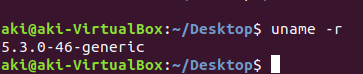
\includegraphics[width=0.7\textwidth]{1.compiling environment.png}
    \end{subfigure}
    \begin{subfigure}[b]{0.49\textwidth}
    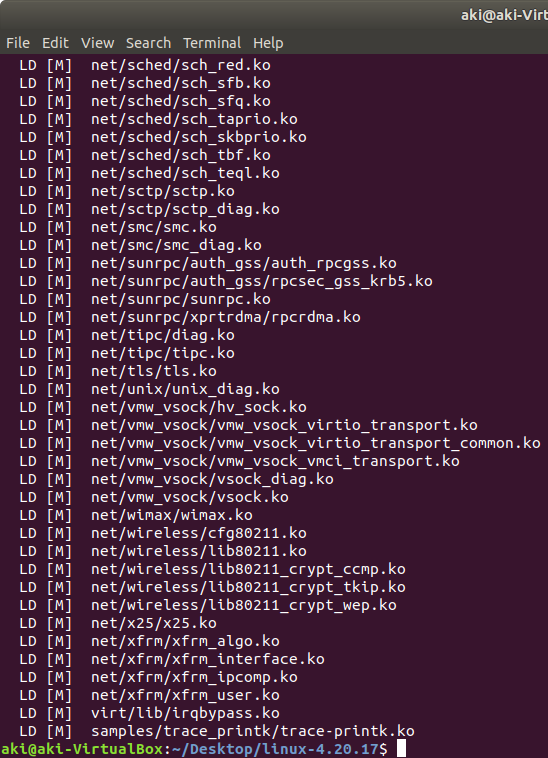
\includegraphics[width=0.7\textwidth]{2.compiling result.png}
    \end{subfigure}
    \caption{Compile and install the compiled Linux kernel.}
\end{figure}

\begin{figure}[ht]
    \centering
    \begin{subfigure}[b]{0.39\textwidth}
    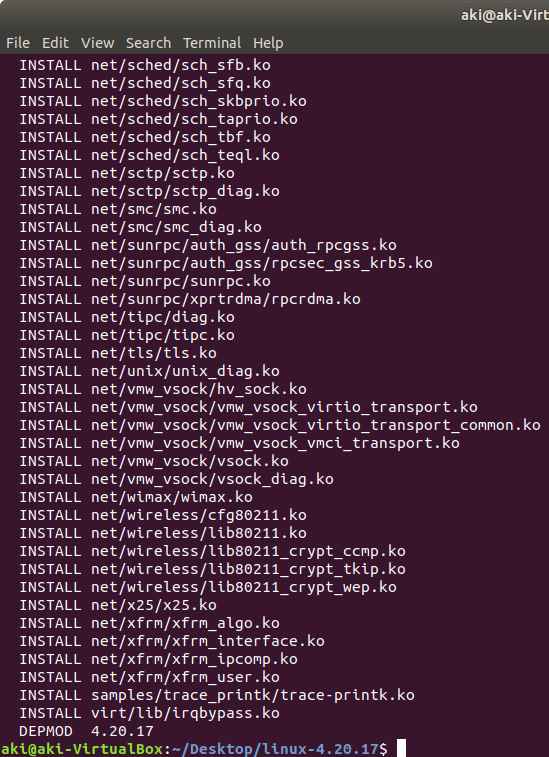
\includegraphics[width=0.73\textwidth]{3.install 1.png}
    \end{subfigure}
    \begin{subfigure}[b]{0.60\textwidth}
    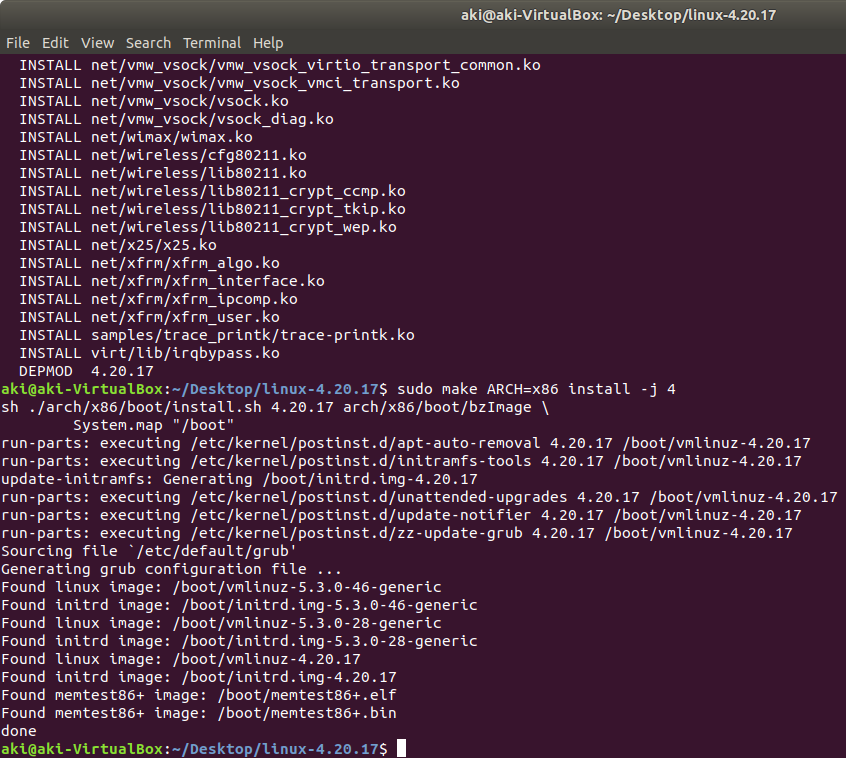
\includegraphics[width=0.73\textwidth]{4.install 2.png}
    \end{subfigure}
    \caption{Install the compiled Linux kernel.}
\end{figure}

\newpage

\section{Loading the Kernel Module and Device Driver Test}

\begin{figure}[ht]
    \centering
    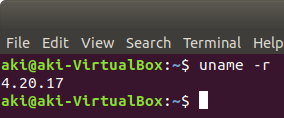
\includegraphics[width=0.5\textwidth]{6.new linux environment.png}
    \caption{New Linux environment.}
\end{figure}

\begin{figure}[ht]
    \centering
    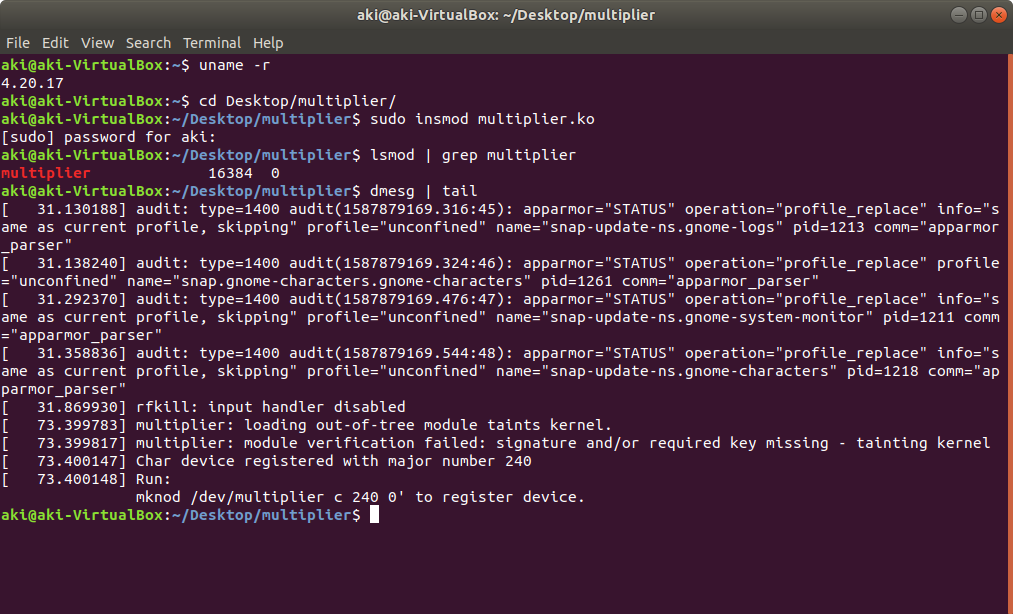
\includegraphics[width=\textwidth]{7.insmod.png}
    \caption{Install the kernel module.}
\end{figure}

\newpage

\begin{figure}[ht]
    \centering
    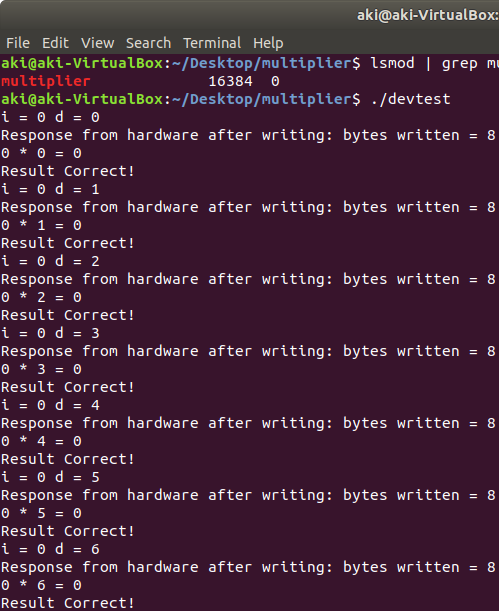
\includegraphics[width=0.32\textwidth]{8.devtest 1.png}
    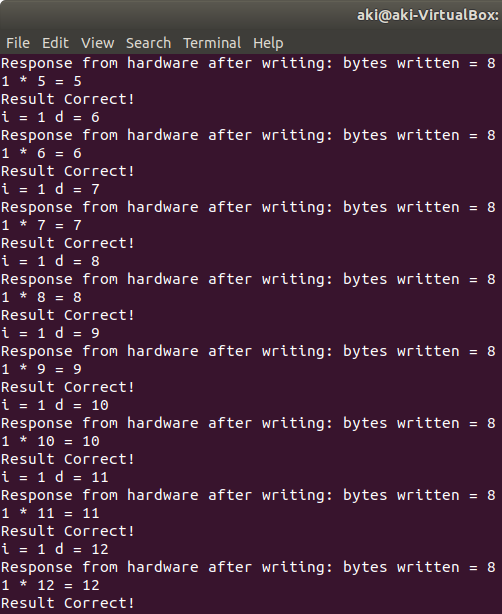
\includegraphics[width=0.32\textwidth]{9.devtest 2.png}
    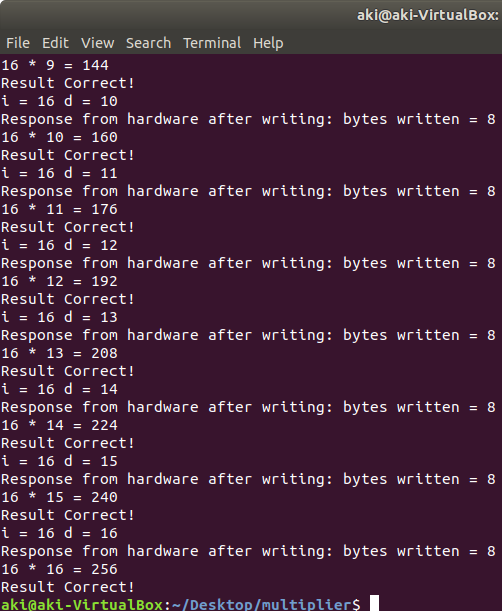
\includegraphics[width=0.32\textwidth]{10.devtest 3.png}
    \caption{Install the compiled Linux kernel.}
\end{figure}

\section{Adding the Kernel Module before Compiling Linux}

\begin{figure}[ht]
    \centering
    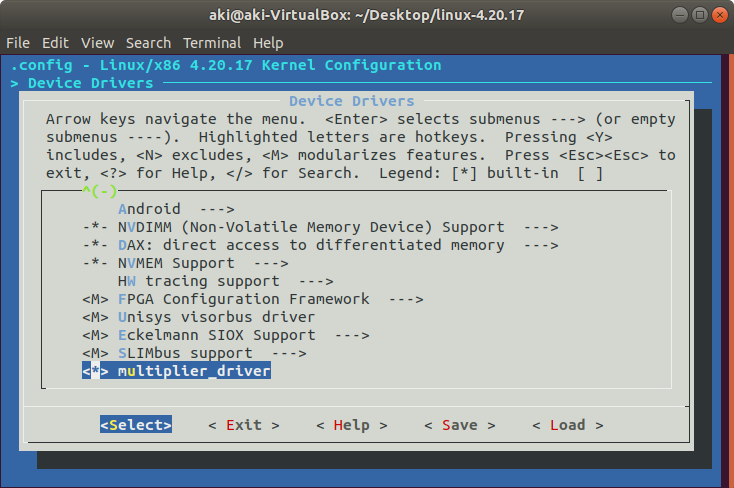
\includegraphics[width=0.7\textwidth]{11.menuconfig multiplier driver.png}
    \caption{Menu configuration for including the multiplier before compiling Linux.}
\end{figure}

\newpage

\section{Device Driver Test with Built-in Module}

\begin{figure}[ht]
    \centering
    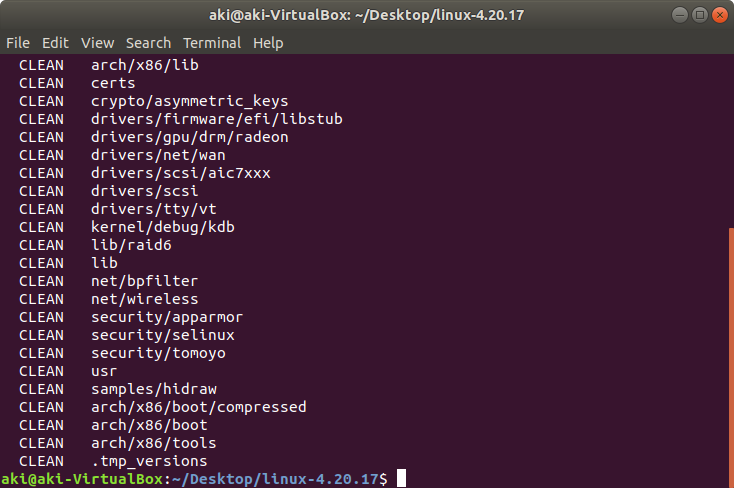
\includegraphics[width=0.65\textwidth]{12.recompiled Linux.png}
    \caption{Linux re-compiled with multiplier module built-in.}
\end{figure}

\begin{figure}[ht]
    \centering
    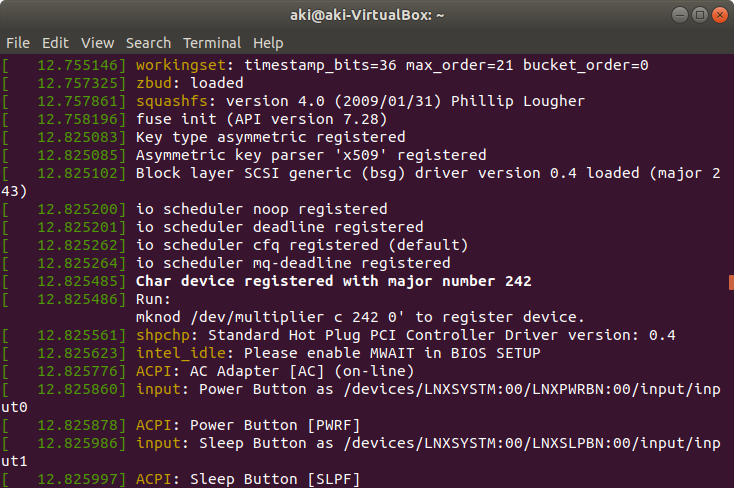
\includegraphics[width=0.65\textwidth]{13.built-in multiplier.png}
    \caption{Linux re-compiled with multiplier module built-in.}
\end{figure}

\newpage

\begin{figure}[ht]
    \centering
    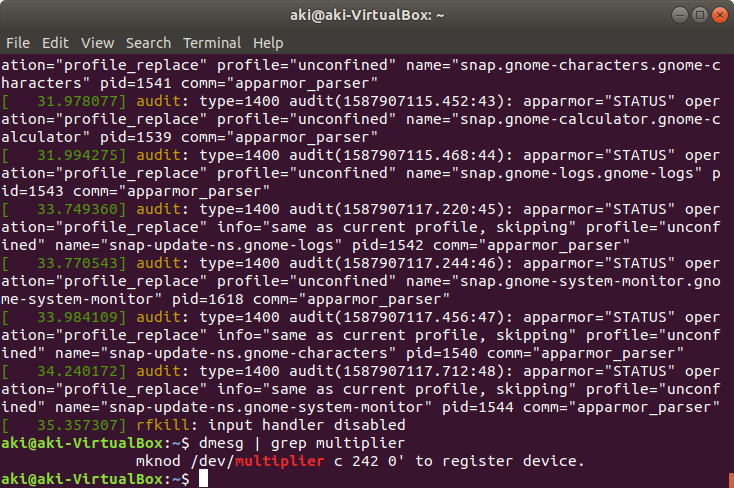
\includegraphics[width=0.65\textwidth]{14.multiplier dmesg.png}
    \caption{dmesg showing the kernel module loaded at boot time.}
\end{figure}

\begin{figure}[ht]
    \centering
    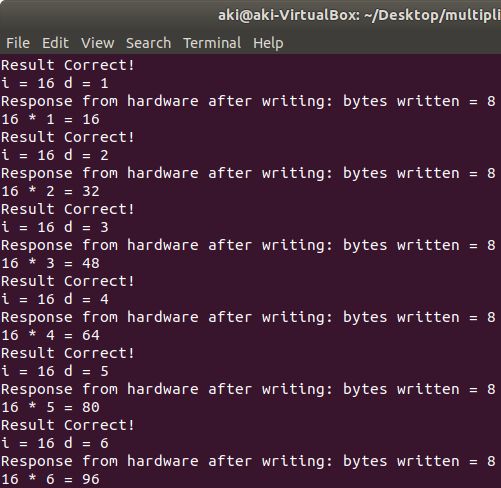
\includegraphics[width=0.45\textwidth]{15.recompiled devtest.png}
    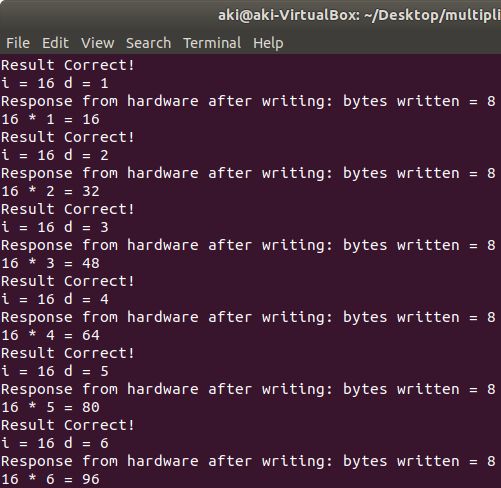
\includegraphics[width=0.45\textwidth]{15.recompiled devtest.png}
    \caption{Running device driver test with multiplier module built-in.}
\end{figure}



\newpage

\part{Conclusion}

The compiled Linux kernel with or without the multiplier built-in all have the size of 8,603,520 bytes. One explanation may be the compiler optimizes the kernel size. Or the multiplier module may be too small to be significant compared with the whole Linux kernel.

\textbf{Q: What are the advantages and disadvantages of both the loadable kernel modules and
built-in module approach?}

A: Advantage of loadable kernel modules:

\begin{enumerate}
    
    \item The kernel module can be easily re-compiled after modification.
    
    \item Can reduce the size of the Linux kernel.
    
    \item Can easily add or remove the module if needed. No need to re-compile the whole Linux kernel which requires a lot of time.
    
\end{enumerate}

Disadvantage of loadable kernel modules:

\begin{enumerate}
    
    \item Need additional configuration on the base Linux kernel if the module is needed.
    
    \item Loading a new kernel module may conflict with other modules or have compatibility issues.
    
    \item Being hot-loadable may reduce the performance: compile the Linux kernel with module built-in may enable the compiler to do some optimization that increases the performance. Being hot-loadable may cause some compromise between performance and flexibility.
    
\end{enumerate}

Advantage of built-in modules:

\begin{enumerate}
    
    \item Need no extra configuration. The kernel is ready to use out of the box.
    
    \item Will not cause compatibility issues: a well-tested Linux kernel will undergo thorough tests to eliminate any chance of interference between modules.
    
    \item Compiler may optimize the module performance or the size taken in the kernel.
    
\end{enumerate}

Disadvantage of built-in modules:

\begin{enumerate}
    
    \item Size of the Linux kernel increases. Depends on the size of the module, may cause significant extra time in distributing the Linux kernel, i.e. downloading the kernel from a FTP site.
    
    \item May need to re-compile the whole Linux kernel if the module undergoes upgrade or bug-fix that can take a long time.
    
\end{enumerate}

\newpage

\textbf{Q: Describe both one good thing and one thing that can be improved about your experience
in the labs this semester.}

A: One good thing: the progressive learning curve presented across the different lab sessions is great. Students learn from the most basic and the easiest and move to the more difficult problem. Some labs are connected so students will not forget those lab sessions after submitting the lab reports.

One thing that can be improved: can have bonus parts in each lab. Such bonus parts need not to count towards the final grade. Students who finish their labs early or are truly interested in areas like FPGA or digital design may be interested in doing such bonus parts to enhance the communication with the instructor and expand their knowledge if they have any plans about the related areas in the future.

\newpage

\begin{appendices}

\section{Makefile}
\label{appendix:makefile}
\lstinputlisting[style={txt-style}]{Makefile}

\section{multiplier.h}
\label{appendix:sourcecode_multiplier_header}
\lstinputlisting[style={txt-style}]{multiplier.h}

\section{multiplier.c}
\label{appendix:sourcecode_multiplier}
\lstinputlisting[style={txt-style}]{multiplier.c}

\section{devtest.c}
\label{appendix:sourcecode_devtest}
\lstinputlisting[style={txt-style}]{devtest.c}

\end{appendices}

\end{document}
